\documentclass[8pt, a4paper, oneside, twocolumn]{extarticle}
\usepackage{graphicx}
\usepackage[export]{adjustbox}
\usepackage[compact]{titlesec}  % documentation: http://mirror.iopb.res.in/tex-archive/macros/latex/contrib/titlesec/titlesec.pdf  
\usepackage{kotex}
\usepackage[left=0.8cm, right=0.8cm, top=2cm, bottom=0.3cm, a4paper]{geometry}
\usepackage{amsmath}
\usepackage{ulem}
\usepackage{amssymb}
\usepackage{minted}  % syntax highlighting
\usepackage{enumitem}
\setlist{nolistsep}
\usepackage{fancyhdr} % documentation: http://ctan.math.utah.edu/ctan/tex-archive/macros/latex/contrib/fancyhdr/fancyhdr.pdf
\usepackage{lastpage}  % just so that we can use \pageref {LastPage}
\usepackage{color, hyperref}
% The lines in the table of contents become links to the corresponding pages in the document by simply adding in the preamble of the document the line
\usepackage{tikz}
\usetikzlibrary{positioning,chains,fit,shapes,calc}
\newcommand{\swastik}[1]{%
    \begin{tikzpicture}[#1]
        \draw (-1,1)  -- (-1,0) -- (1,0) -- (1,-1);
        \draw (-1,-1) -- (0,-1) -- (0,1) -- (1,1);
    \end{tikzpicture}%
}
\newcommand{\revised}{To be \textcolor{red}{\textbf{revised}}.}
\titlespacing*{\section}
{0pt}{0px plus 1px minus 0px}{-2px plus 0px minus 0px}
\titlespacing*{\subsection}
{0pt}{0px plus 1px minus 0px}{0px plus 3px minus 3px}
\titlespacing*{\subsubsection}
{0pt}{0px plus 1px minus 0px}{0px plus 3px minus 3px}
\setlength{\columnseprule}{0.4pt}
\DeclareRobustCommand{\stirling}{\genfrac\{\}{0pt}{}}
\setlength{\parindent}{0pt}  % so that there is no indent of paras.
\begin{document}
\title{\swastik {scale = 0.2} {}Compiler Short Revision Notes{} \swastik {scale = 0.2}}
\author{Sourabh Aggarwal}
\date{Compiled on \today}
\maketitle
\pagenumbering{roman}
\tableofcontents
\newpage
\thispagestyle{fancy}  % else it was not giving fancy header to the first page
\pagenumbering{arabic}
\section{Intro}
Lexical means relating to the words or vocabulary of a language.

Most useful abstraction are context free grammer for parsing and regular expressions for lexical analysis. Yacc which converts a grammer into a parsing program, Lex which converts a declarative specification into lexical analysis program. 

Useful resource: \href{https://www.cs.princeton.edu/~appel/modern/ml/}{Click}

Language of straight line programs:

The informal semantics of the language is as follows. Each $Stm$ is a 
statement, each $Exp$ is an expression. $s_1;s_2$ executes statement $s_1$, then statement
$s_2$. i:=e evaluates the expression e, then "stores" the result in variable i.

print ($e_1, e_2, \dots, e_n$) displays the values of all the expressions, evaluated
left to right, separated by spaces, terminated by a newline.
An identifier expression, such as i, yields the current contents of the 
variable i. A number evaluates to the named integer. An operator expression
$e_1 \text{ op } e_2$ evaluates e1, then e2, then applies the given binary operator. And
an expression sequence (s, e) behaves like the C-language "comma" 
operator, evaluating the statement s for side effects before evaluating (and returning
the result of) the expression e.
For example, executing this program
a := 5+3; b := (print(a, a-1), 10*a); print(b)
prints

8 7

80

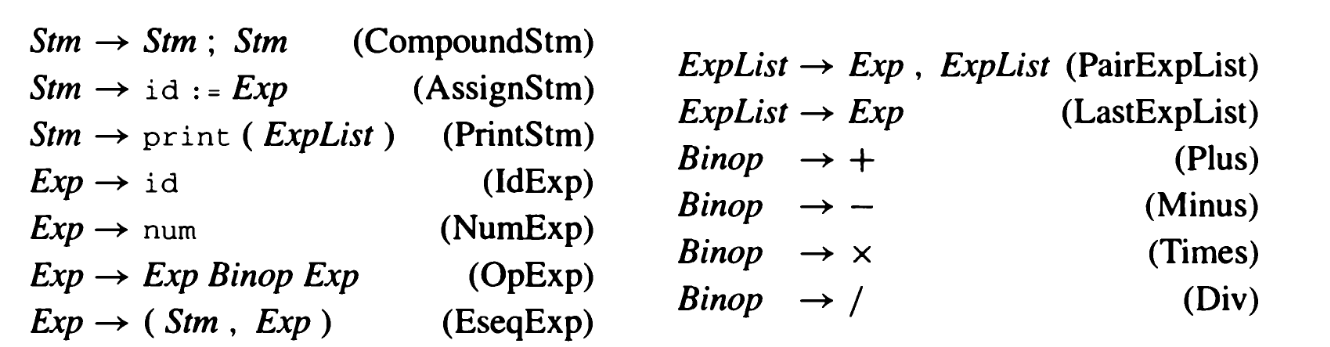
\includegraphics[width=0.5\textwidth,height=0.5\textheight,keepaspectratio]{slpg}

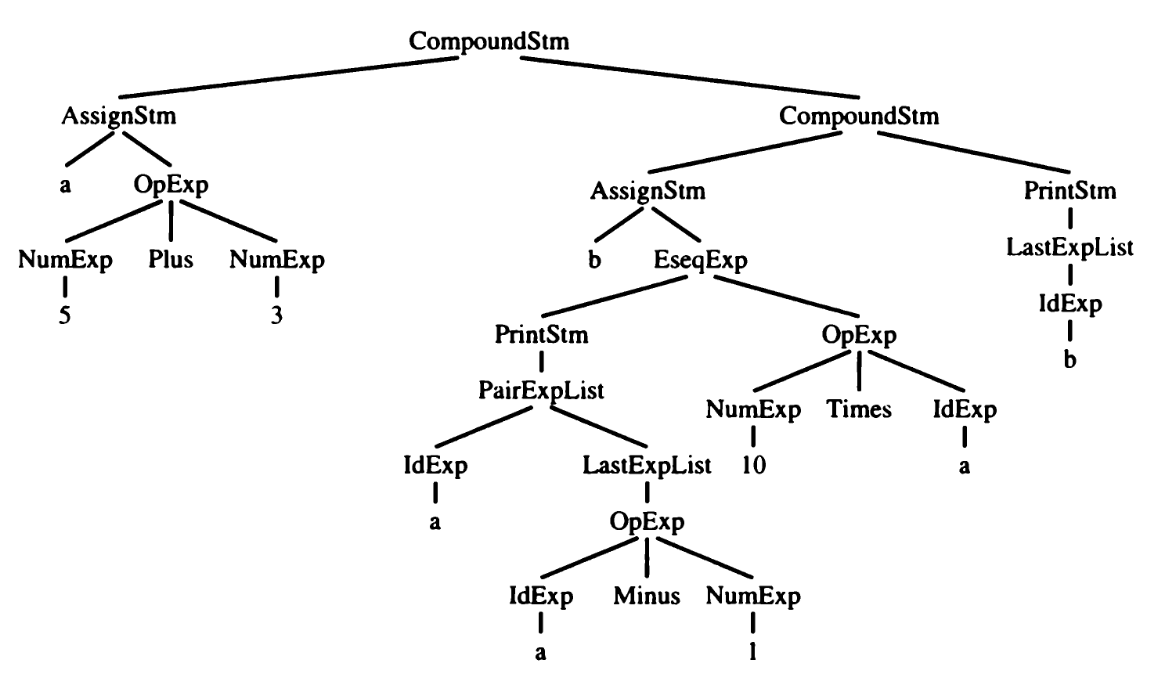
\includegraphics[width=0.5\textwidth,height=0.5\textheight,keepaspectratio]{slpt}

\begin{minted}{SML}
type id = string
datatype binop = Plus | Minus | Times | Div
datatype stm = CompoundStm of stm * stm
             | AssignStm of id * exp
             | PrintStm of exp list
     and exp = IdExp of id
             | NumExp of int
             | OpExp of exp * binop * exp
             | EseqExp of stm * exp
\end{minted}
To translate a program from one language into another, a compiler must first 
pull it apart and understand its structure and meaning, then put it together in a 
different way. The front end of the compiler performs analysis; the back end 
does synthesis. 
The analysis is usually broken up into 
Lexical analysis: breaking the input into individual words or "tokens";The lexical analyzer takes a stream of characters and produces a stream of 
names, keywords, and punctuation marks;  it discards white space and comments between the tokens. 

Syntax analysis: parsing the phrase structure of the program; and 

Semantic analysis: calculating the program's meaning. 

we will specify lexical tokens using the formal language of regular 
expressions, implement lexers using deterministic finite automata, and use 
mathematics to connect the two. This will lead to simpler and more readable 
lexical analyzers. 
$(a \odot b) \vert \epsilon$ represents the language \{""," ab"\}. 
In writing regular expressions, we will sometimes omit the concatenation 
symbol or the epsilon, and we will assume that Kleene closure "binds tighter" 
than concatenation, and concatenation binds tighter than alternation; so that 
$ab \vert c$ means $(a \odot b) \vert c$, and $(a \vert)$ means $(a \vert \epsilon)$. 
Let us introduce some more abbreviations: [abed] means 
$(a \vert b \vert c \vert 
d)$, [b-g] means [bedefg], [b-gM-Qkr] means [bcdefgMNOPQkr], M? 
means ($M \vert \epsilon$), and $M^+$ means ($M \odot M^*$). 

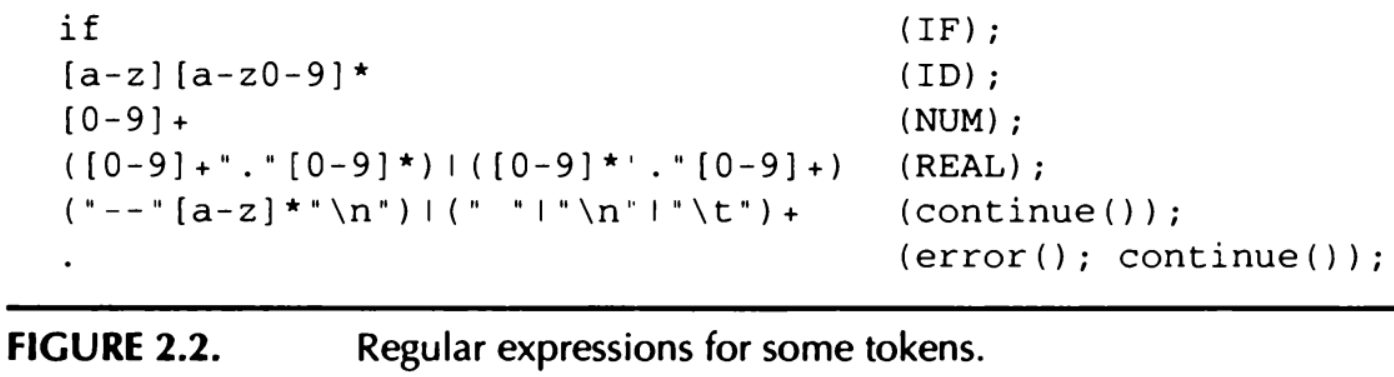
\includegraphics[width=0.5\textwidth,height=0.5\textheight,keepaspectratio]{reg}

Longest match: The longest initial substring of the input that can match any 
regular expression is taken as the next token. 

Rule priority: For a particular longest initial substring, the first regular  
expression that can match determines its token type. This means that the order of 
writing down the regular-expression rules has significance. 

So according to the rules, if8 match as a single 
identifier and not as the two tokens if and 8. And "if 89" begin with a 
reserved word and not by an identifier by rule priority rule. 

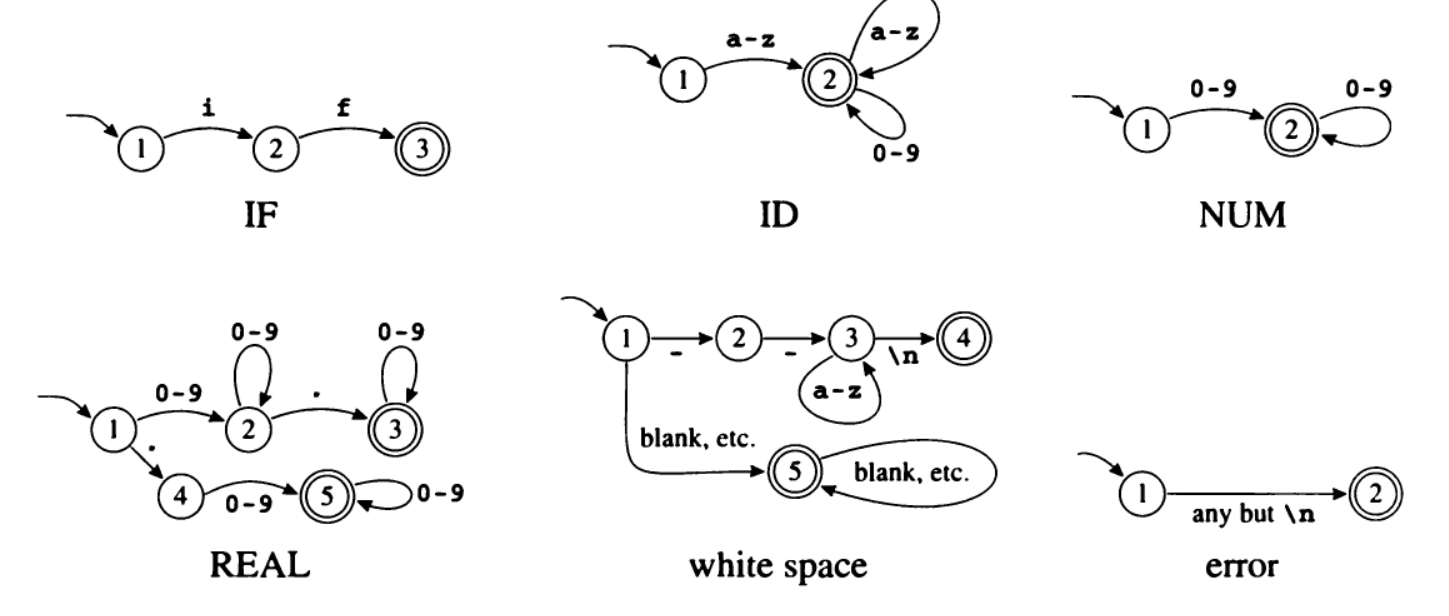
\includegraphics[width=0.5\textwidth,height=0.5\textheight,keepaspectratio]{aut}

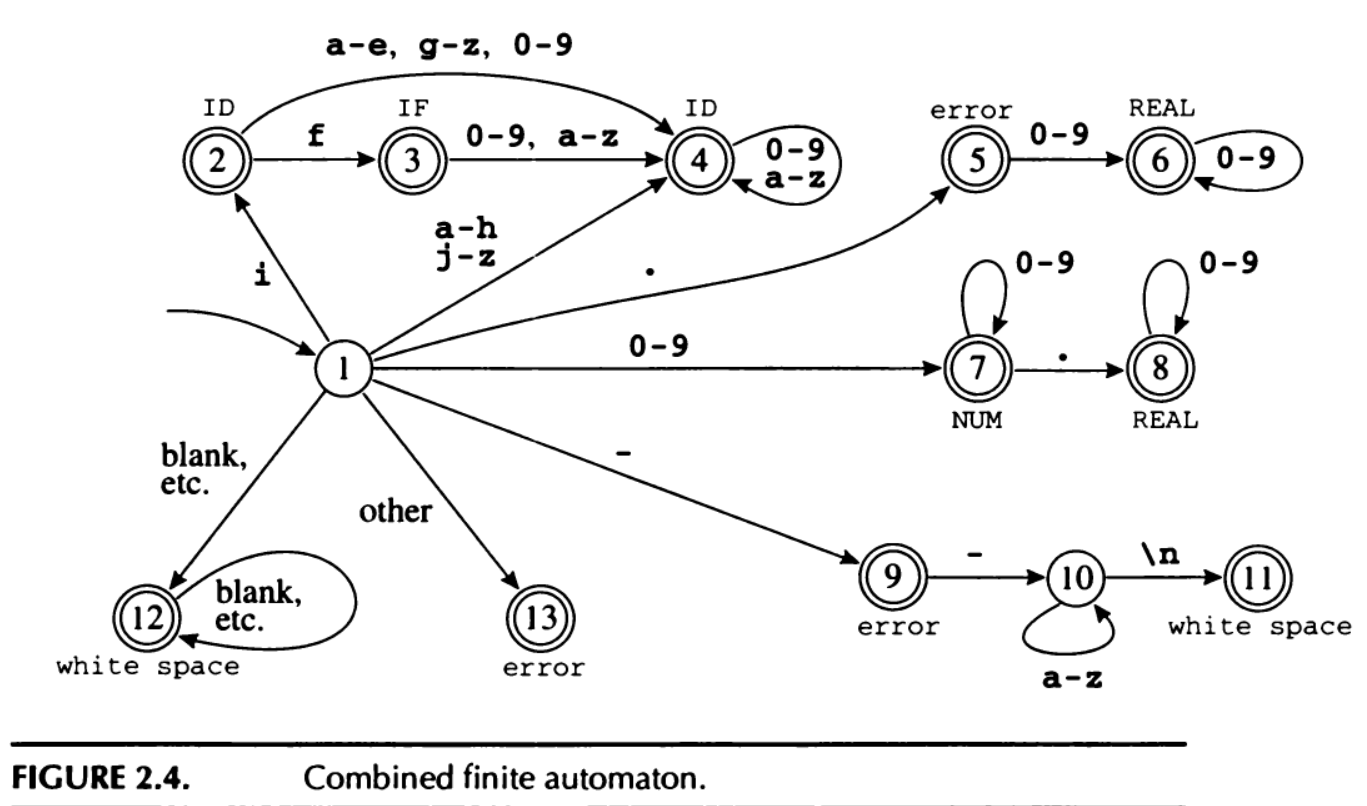
\includegraphics[width=0.5\textwidth,height=0.5\textheight,keepaspectratio]{cfa}

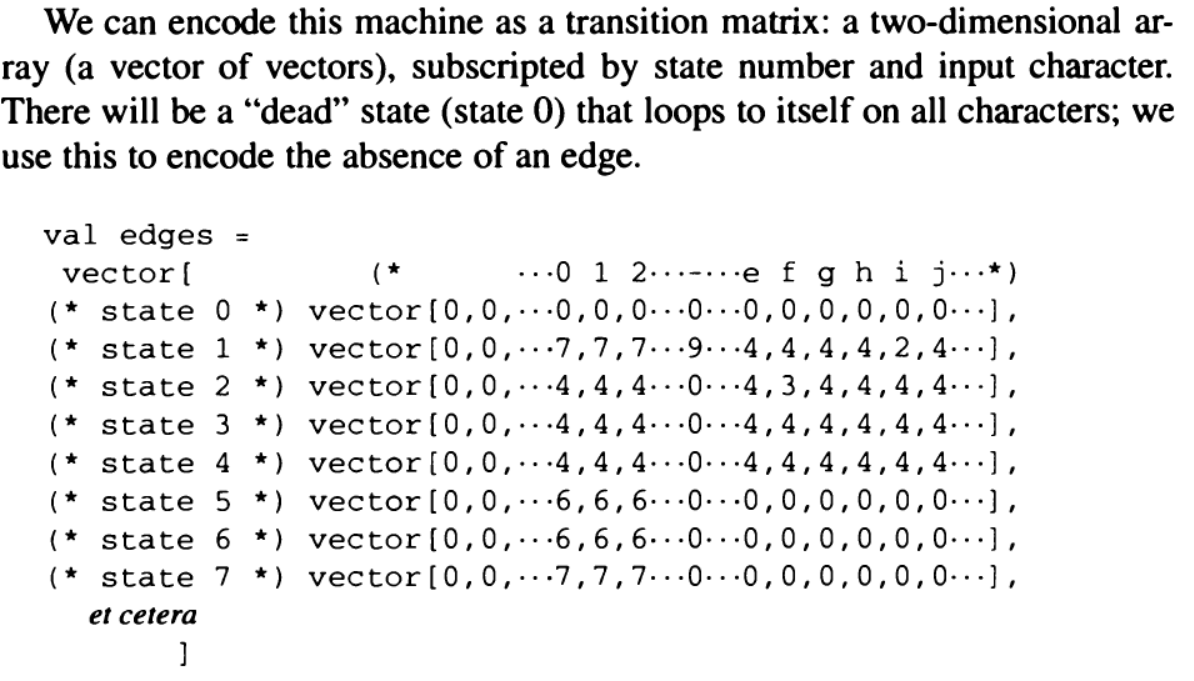
\includegraphics[width=0.5\textwidth,height=0.5\textheight,keepaspectratio]{mat}

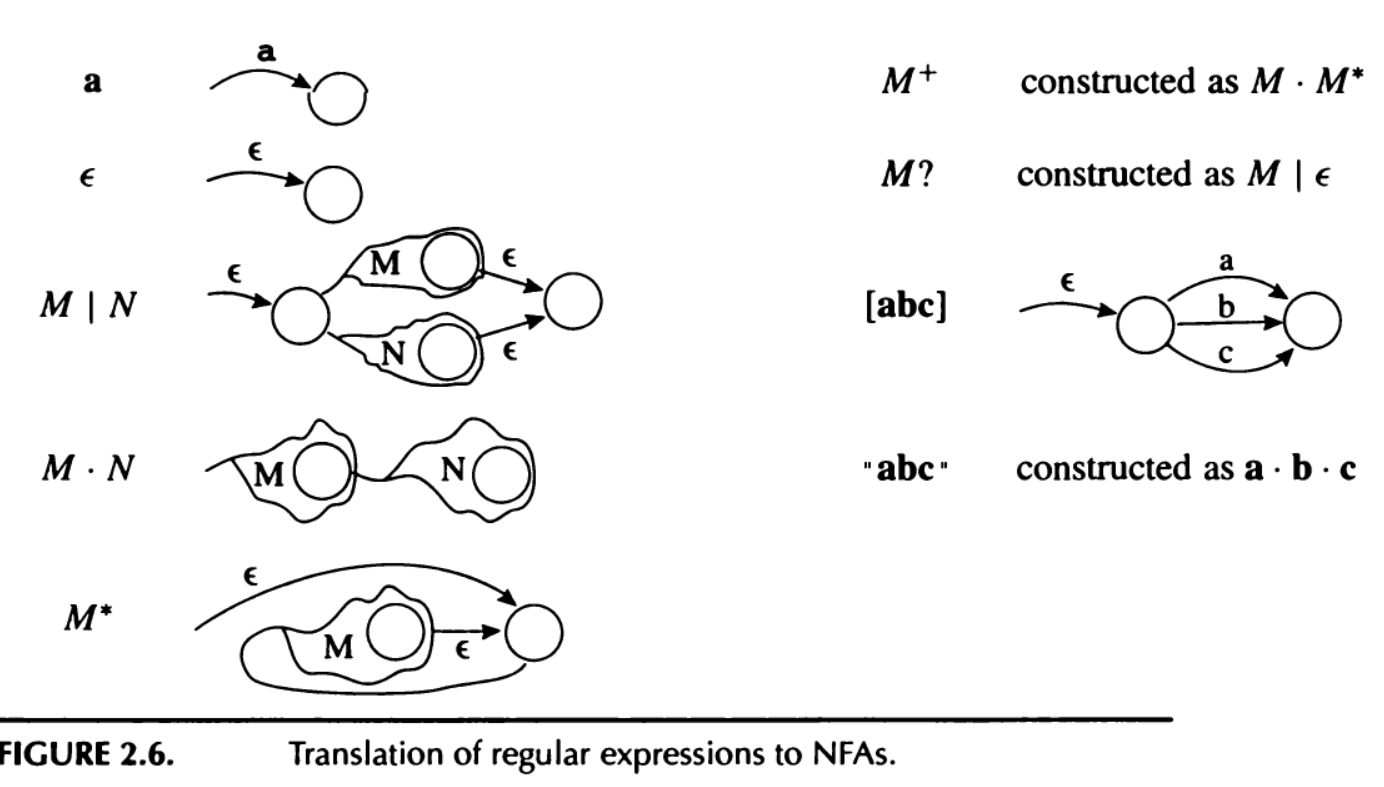
\includegraphics[width=0.5\textwidth,height=0.5\textheight,keepaspectratio]{rtnfa}

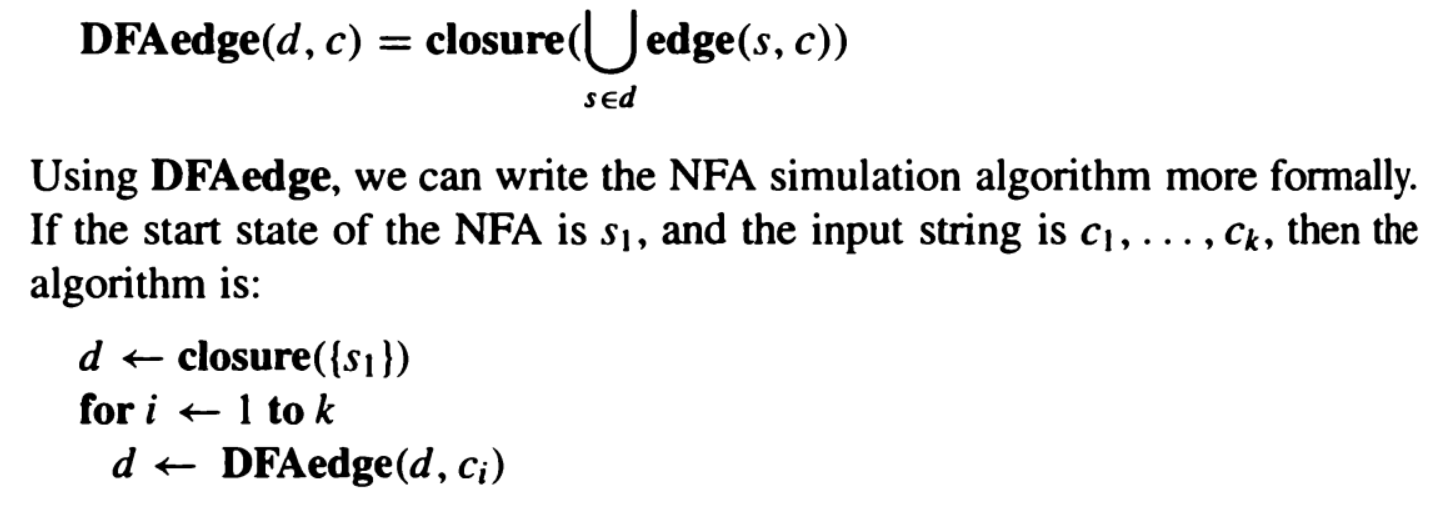
\includegraphics[width=0.5\textwidth,height=0.5\textheight,keepaspectratio]{nfa1}

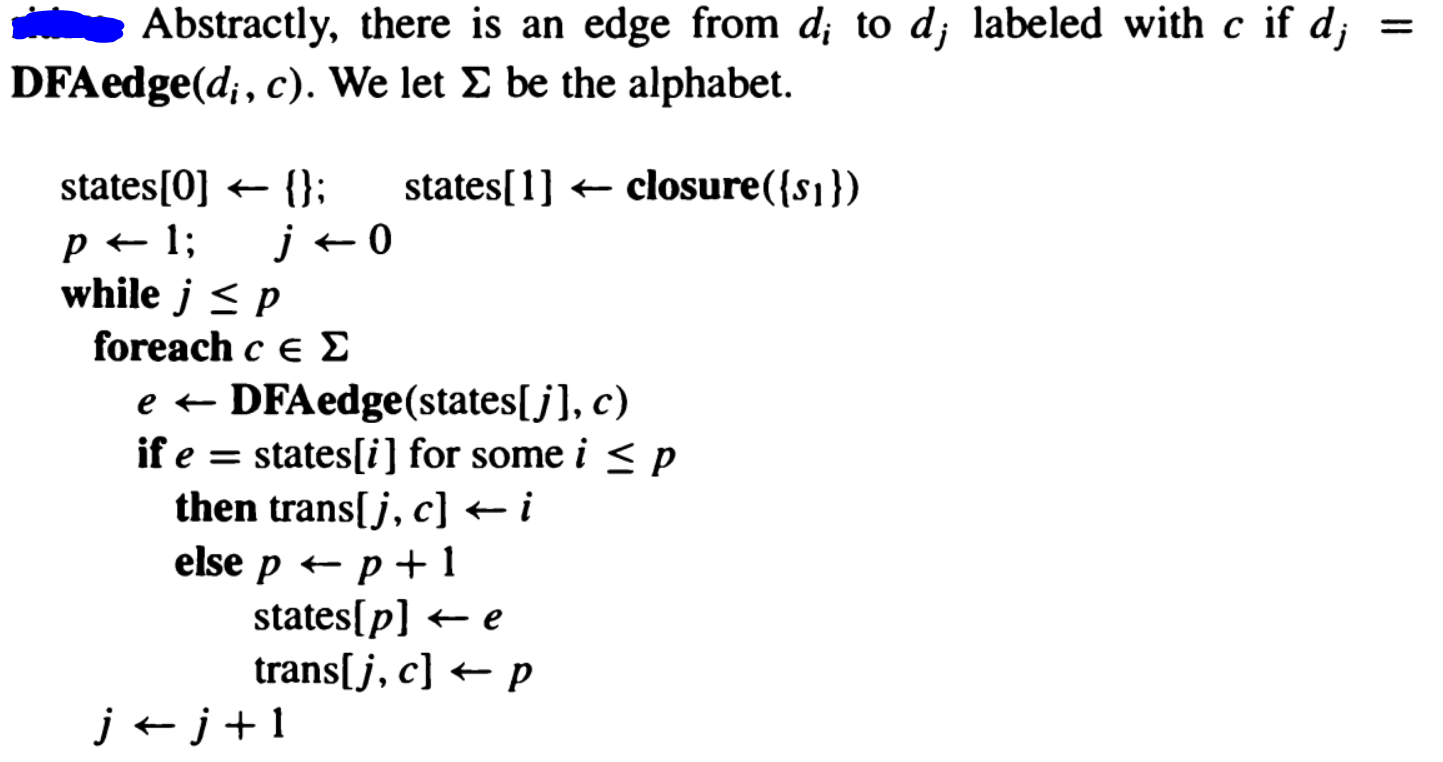
\includegraphics[width=0.5\textwidth,height=0.5\textheight,keepaspectratio]{nfa2}

DFA construction is a mechanical task easily performed by computer, so it 
makes sense to have an automatic lexical analyzer generator to translate  
regular expressions into a DFA. 

ML-Lex is a lexical analyzer generator that produces an ML program from 
a lexical specification. 

For each token type in the programming language to 
be lexically analyzed, the specification contains a regular expression and an 
action. The action communicates the token type (perhaps along with other 
information) to the next phase of the compiler. 

The output of ML-Lex is a program in ML - a lexical analyzer that  
interprets a DFA using the algorithm described in Section 2.3 and executes the 
action fragments on each match. The action fragments are just ML statements 
that return token values. 

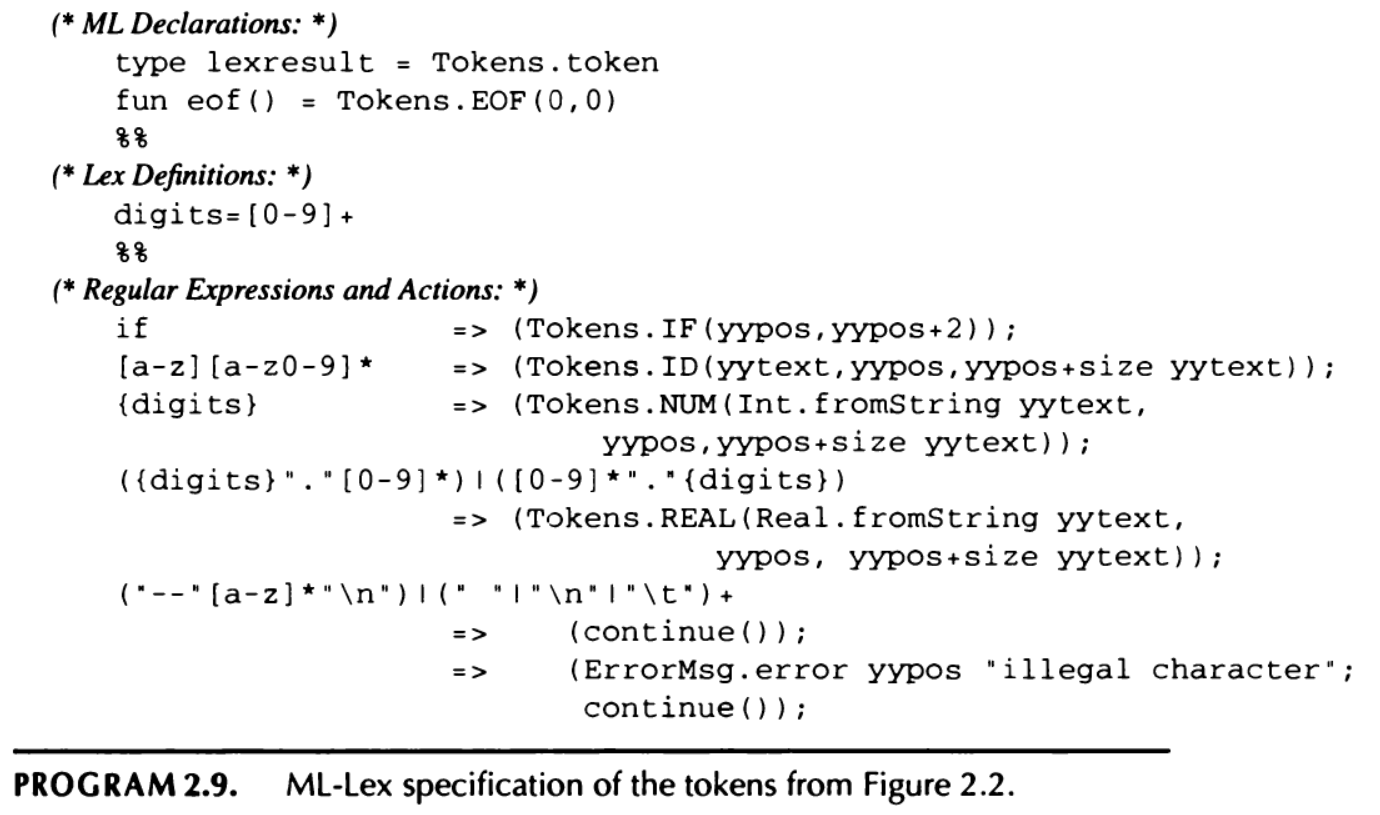
\includegraphics[width=0.5\textwidth,height=0.5\textheight,keepaspectratio]{lex}

The first part of the specification, above the first \%\% mark, contains  
functions and types written in ML. These must include the type lexresult, 
which is the result type of each call to the lexing function; and the  
function eof, which the lexing engine will call at end of file. This section can 
also contain utility functions for the use of the semantic actions in the third 
section. 

The second part of the specification contains regular-expression  
abbreviations and state declarations. For example, the declaration digits=$[0-9]^+$ 
in this section allows the name \{digits\} to stand for a nonempty sequence 
of digits within regular expressions. 

The third part contains regular expressions and actions. The actions are 
fragments of ordinary ML code. Each action must return a value of type 
lexresult. In this specification, lexresult is a token from the Tokens 
structure. 

In the action fragments, several special variables are available. The string 
matched by the regular expression is yytext. The file position of the  
beginning of the matched string is yypos. The function continue () calls the 
lexical analyzer recursively. 

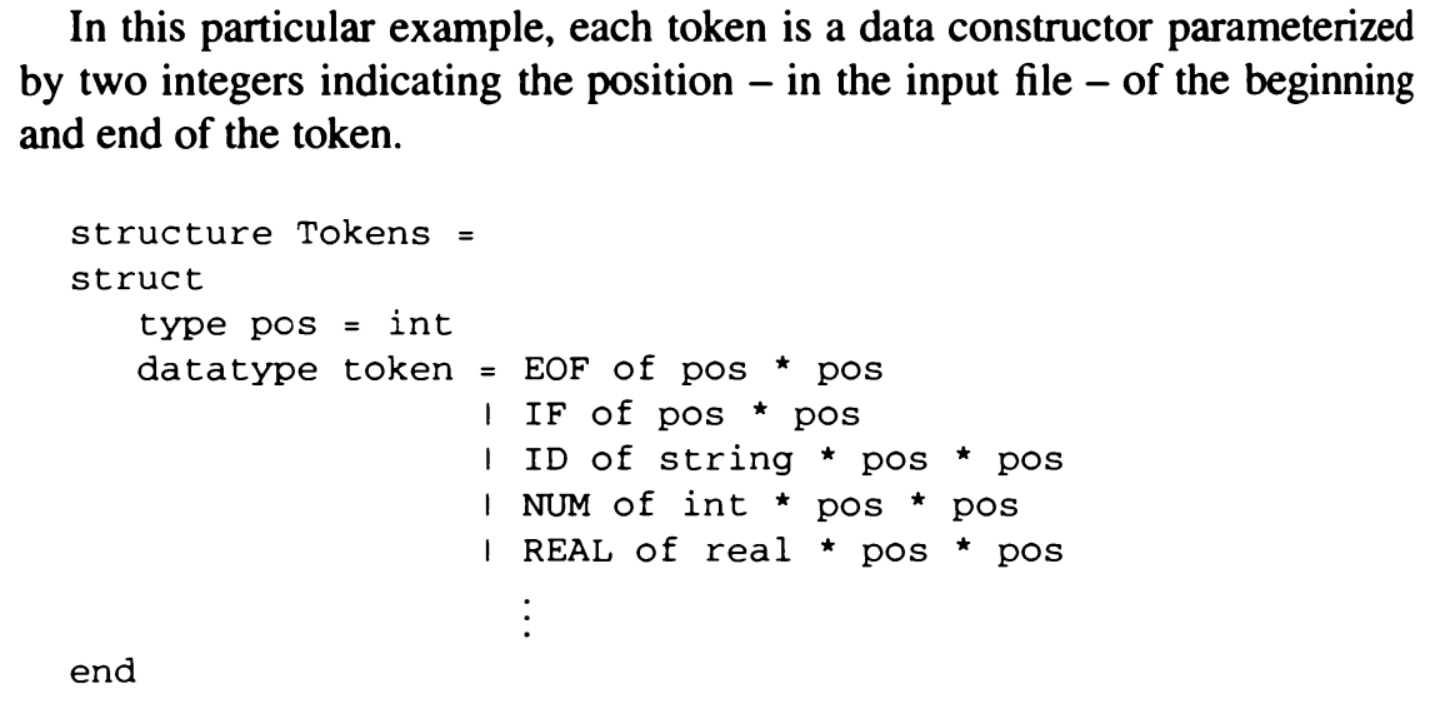
\includegraphics[width=0.5\textwidth,height=0.5\textheight,keepaspectratio]{lex2}

But sometimes the step-by-step, state-transition model of automata is  
appropriate. ML-Lex has a mechanism to mix states with regular expressions. 
One can declare a set of start states; each regular expression can be prefixed 
by the set of start states in which it is valid. The action fragments can  
explicitly change the start state. In effect, we have a finite automaton whose edges 
are labeled, not by single symbols, but by regular expressions. This example 
shows a language with simple identifiers, if tokens, and comments delimited 
by (* and *) brackets: 

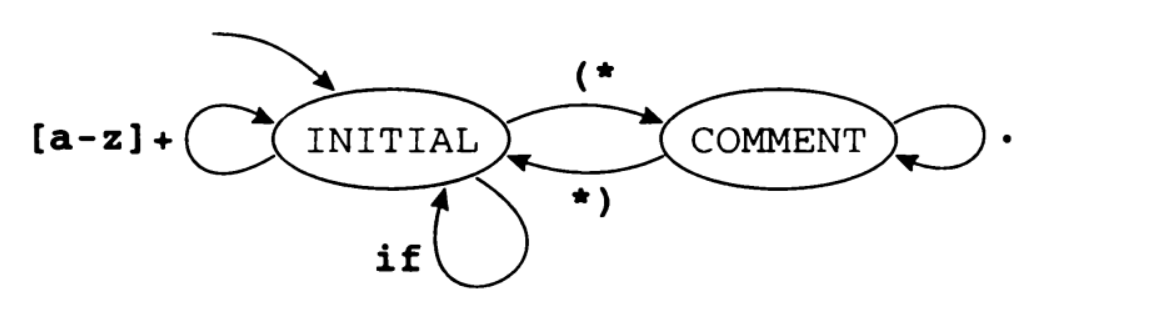
\includegraphics[width=0.5\textwidth,height=0.5\textheight,keepaspectratio]{lex3}

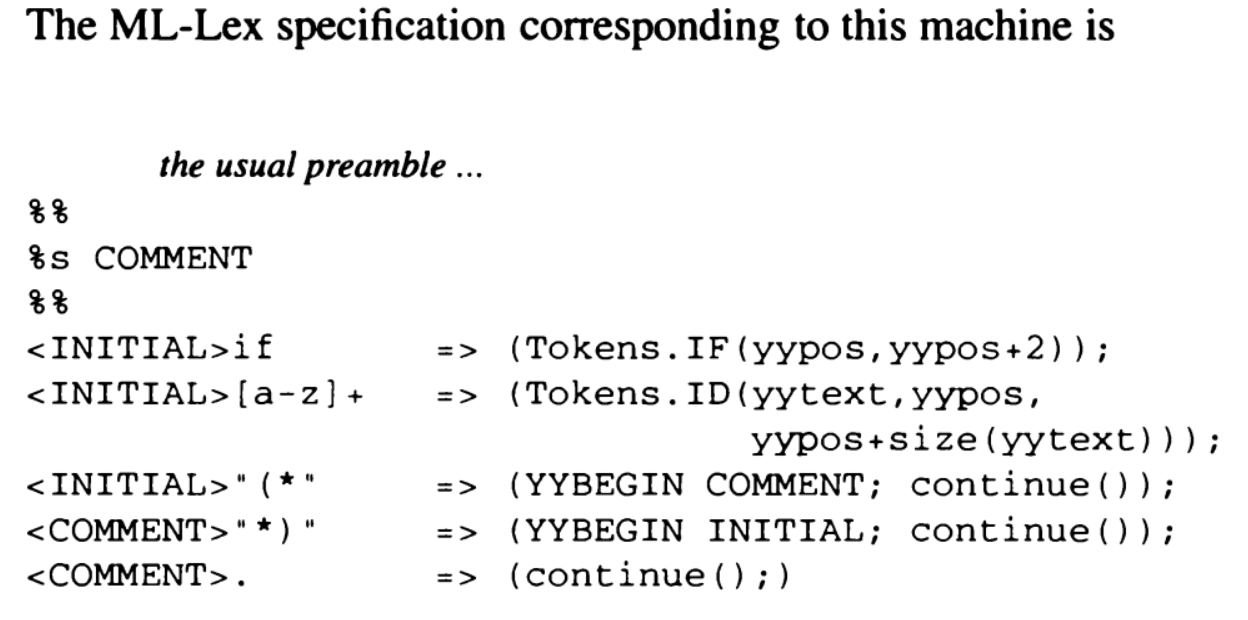
\includegraphics[width=0.5\textwidth,height=0.5\textheight,keepaspectratio]{lex4}

This example can be easily augmented to handle nested comments, via a 
global variable that is incremented and decremented in the semantic actions. 

Any regular expression not prefixed by a $<state>$ operates in all states; this  
feature is rarely useful. 

\end{document}